% Chapter 8. The control-flow inversion, before and after.
\documentclass[tikz,border=6pt]{standalone}
% Shared look for every TikZ figure in the book.
% Colours match book/preamble.tex exactly. Change both or neither.

\usepackage{tikz}
\usepackage{xcolor}
\usepackage{amsmath}
\IfFileExists{libertinus.sty}{\usepackage[mono=false]{libertinus}}{}
\IfFileExists{inconsolata.sty}{\usepackage[varqu,varl,scaled=0.95]{inconsolata}}{}

\usetikzlibrary{
  arrows.meta, positioning, calc, fit, backgrounds, shapes.geometric,
  shapes.misc, decorations.pathreplacing, decorations.pathmorphing,
  patterns, chains, matrix, shadows.blur
}

\definecolor{ink}{HTML}{15181D}
\definecolor{muted}{HTML}{5B6472}
\definecolor{rule}{HTML}{C9CED6}
\definecolor{wash}{HTML}{F4F5F7}
\definecolor{accent}{HTML}{0F5C8C}
\definecolor{accentsoft}{HTML}{E7F0F6}
\definecolor{warm}{HTML}{B4531A}
\definecolor{warmsoft}{HTML}{FBF0E7}
\definecolor{good}{HTML}{2C6E49}
\definecolor{goodsoft}{HTML}{E9F2EC}
\definecolor{danger}{HTML}{9B2226}
\definecolor{dangersoft}{HTML}{FAECEC}

\tikzset{
  font=\sffamily\small,
  >={Stealth[length=5pt, width=4pt]},
  %
  box/.style={
    draw=rule, line width=0.8pt, fill=wash, rounded corners=2pt,
    inner sep=7pt, align=center, text=ink, minimum height=9mm,
  },
  boxa/.style={box, draw=accent, fill=accentsoft},
  boxg/.style={box, draw=good,   fill=goodsoft},
  boxw/.style={box, draw=warm,   fill=warmsoft},
  boxd/.style={box, draw=danger, fill=dangersoft},
  %
  lane/.style={draw=rule, line width=0.7pt, fill=white, rounded corners=2pt,
               inner sep=6pt, align=center, minimum width=26mm},
  %
  flow/.style={draw=accent, line width=1.0pt, ->},
  flowback/.style={flow, densely dashed},
  flowmuted/.style={draw=muted, line width=0.8pt, ->},
  lifeline/.style={draw=rule, line width=0.7pt, densely dotted},
  %
  lbl/.style={font=\sffamily\scriptsize, text=muted, inner sep=2pt},
  lblink/.style={font=\sffamily\scriptsize, text=ink, inner sep=2pt},
  tag/.style={font=\ttfamily\scriptsize, text=accent, inner sep=2pt,
              fill=white, inner xsep=3pt},
  note/.style={font=\sffamily\scriptsize\itshape, text=muted, align=left},
  %
  band/.style={draw=none, rounded corners=1pt},
  tick/.style={draw=muted, line width=0.6pt},
}

% A horizontal timeline bar segment: \barseg{x0}{x1}{y}{colour}{label}
\newcommand{\barseg}[5]{%
  \fill[#4, rounded corners=1pt] (#1,#3-0.16) rectangle (#2,#3+0.16);
  \node[lbl, text=white, font=\sffamily\scriptsize\bfseries]
       at ({(#1+#2)/2},#3) {#5};
}

\begin{document}
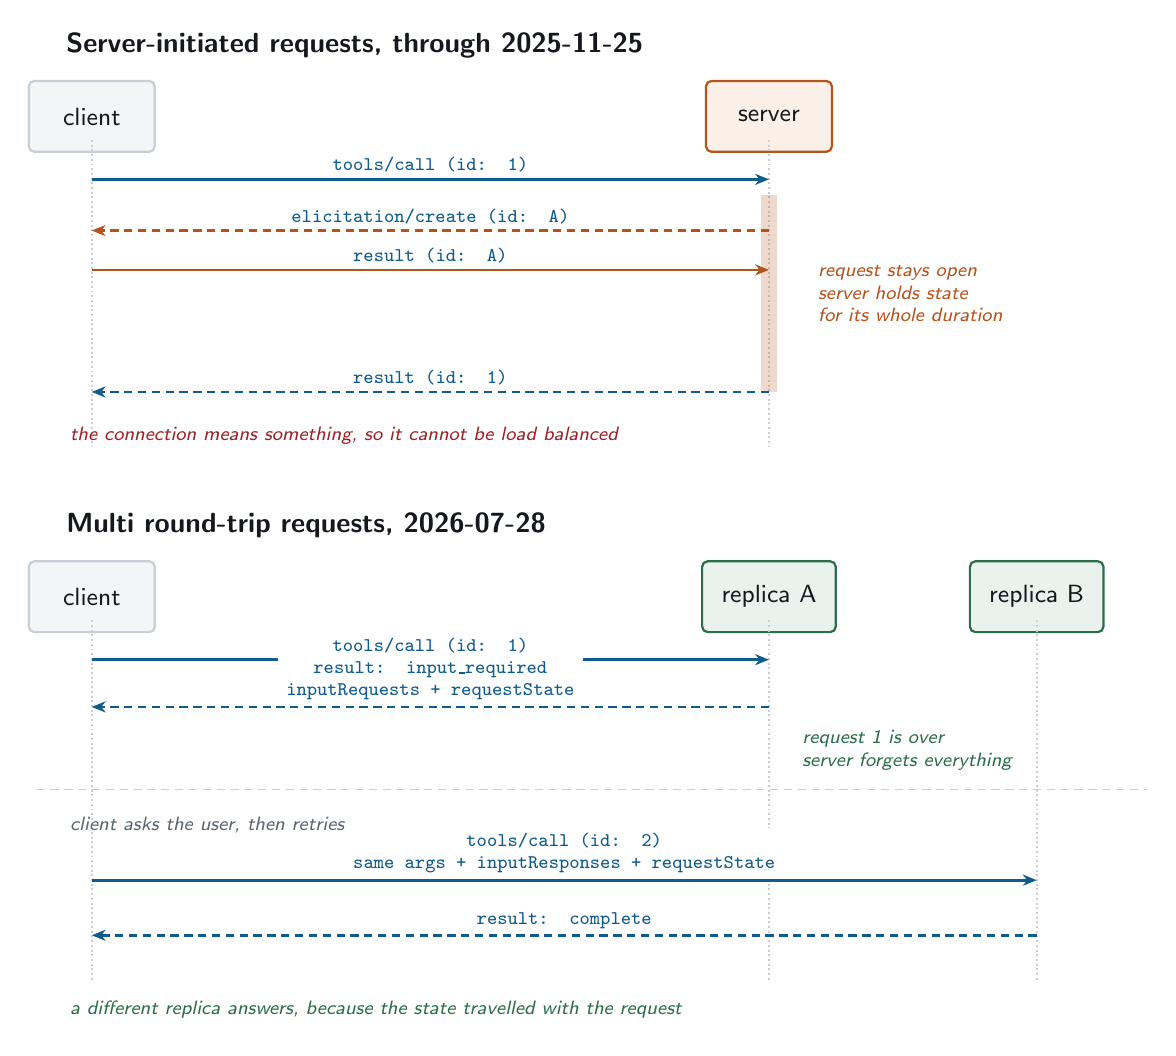
\begin{tikzpicture}[x=1cm, y=1cm]

% =========================================================================
% TOP: server-initiated requests (2025)
% =========================================================================
\begin{scope}[yshift=0cm]
  \node[lblink, font=\sffamily\bfseries, anchor=west] at (-0.4,3.2)
    {Server-initiated requests, through 2025-11-25};

  \node[box,  minimum width=16mm] (c) at (0,2.3) {client};
  \node[boxw, minimum width=16mm] (s) at (8.6,2.3) {server};
  \draw[lifeline] (0,2.0) -- (0,-1.9);
  \draw[lifeline] (8.6,2.0) -- (8.6,-1.9);

  \draw[flow] (0,1.5) -- node[tag, above] {tools/call (id: 1)} (8.6,1.5);

  % the server holds the request open
  \draw[draw=warm, line width=6pt, opacity=0.22] (8.6,1.3) -- (8.6,-1.2);
  \node[note, text=warm, anchor=west, align=left] at (9.1,0.05)
    {request stays open\\server holds state\\for its whole duration};

  \draw[flowback, draw=warm] (8.6,0.85)
        -- node[tag, above] {elicitation/create (id: A)} (0,0.85);
  \draw[flow, draw=warm] (0,0.35) -- node[tag, above] {result (id: A)} (8.6,0.35);
  \draw[flowback] (8.6,-1.2) -- node[tag, above] {result (id: 1)} (0,-1.2);

  \node[note, anchor=west, text=danger, align=left] at (-0.4,-1.75)
    {the connection means something, so it cannot be load balanced};
\end{scope}

% =========================================================================
% BOTTOM: MRTR (2026-07-28)
% =========================================================================
\begin{scope}[yshift=-6.1cm]
  \node[lblink, font=\sffamily\bfseries, anchor=west] at (-0.4,3.2)
    {Multi round-trip requests, 2026-07-28};

  \node[box,  minimum width=16mm] (c2) at (0,2.3) {client};
  \node[boxg, minimum width=16mm] (s2a) at (8.6,2.3) {replica A};
  \node[boxg, minimum width=16mm] (s2b) at (12.0,2.3) {replica B};
  \draw[lifeline] (0,2.0) -- (0,-2.6);
  \draw[lifeline] (8.6,2.0) -- (8.6,-2.6);
  \draw[lifeline] (12.0,2.0) -- (12.0,-2.6);

  \draw[flow] (0,1.5) -- node[tag, above] {tools/call (id: 1)} (8.6,1.5);
  \draw[flowback] (8.6,0.9) -- node[tag, above, align=center]
    {result: input\_required\\\scriptsize inputRequests + requestState} (0,0.9);

  \node[note, anchor=west, text=good, align=left] at (8.9,0.35)
    {request 1 is over\\server forgets everything};

  \draw[draw=rule, line width=0.6pt, densely dashed] (-0.7,-0.15) -- (13.4,-0.15);
  \node[note, anchor=west] at (-0.4,-0.6) {client asks the user, then retries};

  \draw[flow] (0,-1.3) -- node[tag, above, align=center]
    {tools/call (id: \textbf{2})\\\scriptsize same args + inputResponses + requestState} (12.0,-1.3);
  \draw[flowback] (12.0,-2.0) -- node[tag, above] {result: complete} (0,-2.0);

  \node[note, anchor=west, text=good, align=left] at (-0.4,-2.95)
    {a different replica answers, because the state travelled with the request};
\end{scope}

\end{tikzpicture}
\end{document}
